\documentclass[a4paper, 10pt, twocolumn]{article}
\usepackage{amssymb}
\usepackage{cellspace, graphicx, makecell}
\usepackage{graphicx} % Required for inserting images
\usepackage[utf8]{inputenc}
\usepackage[T2A]{fontenc}
\usepackage[english,russian]{babel}
\usepackage{cmap}
\usepackage[left=1cm,right=1cm,
    top=1cm,bottom=2cm]{geometry}
\usepackage{paracol}
\usepackage{multicol}
\usepackage{amsmath}
\usepackage{lipsum}
\usepackage{vwcol}
\usepackage{float}

% Установка размера формул
\DeclareMathSizes{10}{10}{10}{10}   % Для основного текста размером 10pt

\title{Лабораторная работа 3.3.4 \\ Эффект Холла в полупроводниках}
\author{Матвей Галицын \\ Б01-411}
\date{September 5, 2025}

\setlength{\columnseprule}{0.1pt}
\setlength{\columnsep}{3em}
\raggedbottom
\begin{document}
\maketitle
\newpage{}
\section{Аннотация}

\textbf{Цель работы:} измерение подвижности и концентрации носителей заряда в полупроводниках\\

\textbf{В работе используются:} электромагнит с источником питания, амперметр, миллиамперметр, реостат, цифровой вольтметр, источник питания ($1.5 \text{В}$), образцы легированного германия\\

\section{Теория}
    Эффект хола заключается в возникновении разницы потенциалов на поверхности материала при 
    протекании тока через этот материал, если этот материал помещен в магнитное поле. Собственно, в 
    этой работе мы будем помещать образец легированного германия в магнитное поле и измерим 
    зависимость разницы потенциалов между контактами $3-4$ от внешнего поля $B$, вызванного 
    электромагнитами. Также, используя зависимость разницы потенциалов между точками $3-4$ от $I$, 
    мы найдем проводимость $\sigma$, из которой вычеслим постоянную Холла.
\section{Экспериментальная установка}
    \begin{figure}[H]
        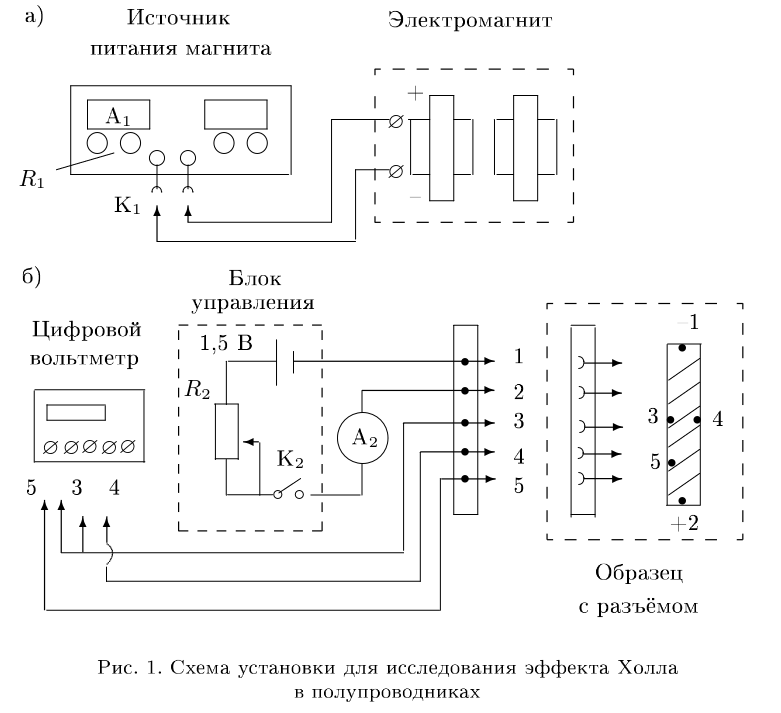
\includegraphics[width=1\linewidth]{images/setup.png}
    \end{figure}
    
\section{Результаты измерений и обработка данных}
    Проверим работу электромагнита и прокалибруем его, измерив зависимость $\Phi$ потока через милливеберметр от тока $I_\text{м}$ через магнит. Из нее найдем поле $B = \Phi / (NS)$, идущее через милливеберметр с $NS = 75\,\text{см}^2$.

    \begin{table}[H]
        \centering
        \begin{tabular}{|l|l|l|l|l|l|l|l|} \hline
        $I$, А & 0.3 & 0.6 & 0.9 & 1.2 & 1.5 & 1.8 & 2.1 \\ \hline
        $\Phi$, мВб & 1.4 & 2.6 & 3.7 & 4.7 & 5.1 & 5.9 & 6.9 \\ \hline
        $B$, мТл & 186 & 347 & 493 & 627 & 680 & 787 & 920 \\ \hline
        \end{tabular}
        \caption{Калибровка магнита}
    \end{table}
    $\Delta I=0.005\,\text{A}, \Delta \Phi=1.5\,\text{мВб}, \Delta B=13\,\text{мТл}$

    \begin{figure}[H]
        \centering
        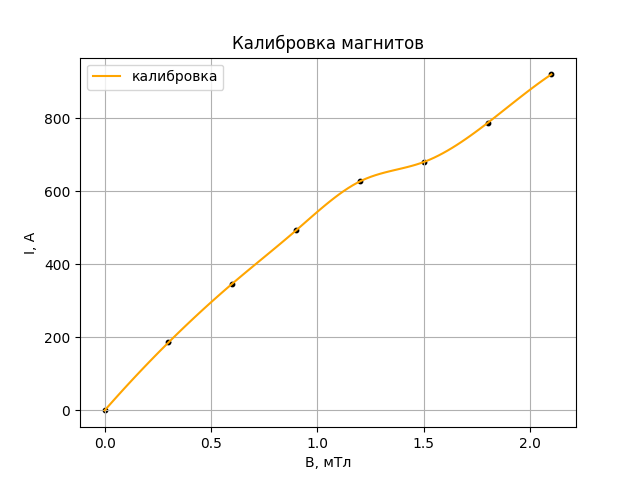
\includegraphics[width=1\linewidth]{graphs/figure1.png}
    \end{figure}

    Измерим ЭДС Холла. Для фиксированного тока через образец $I$ в электромагните измерим зависимость напряжения $U_{34}$ от тока $I_M$ на электромагните.

    Значения приведены в приложении.

    \begin{figure}[H]
        \centering
        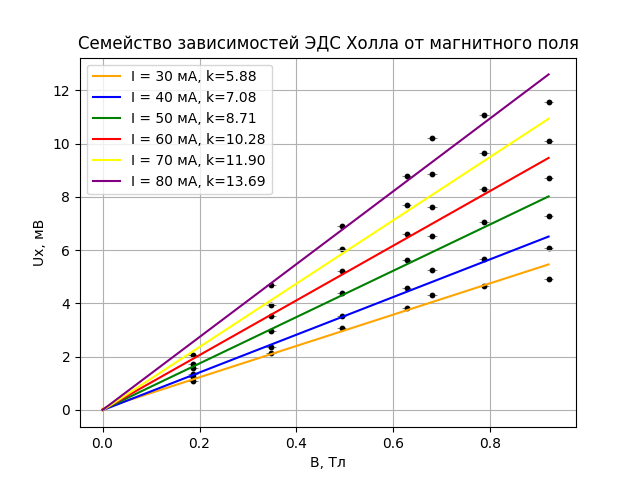
\includegraphics[width=1\linewidth]{graphs/figure2.png}
        \begin{center}
            \caption{Семейство зависимостей ЭДС Холла от магнитного поля в электромагните при разных токах через образец}
        \end{center}
    \end{figure}
    
    \begin{figure}[H]
        \centering
        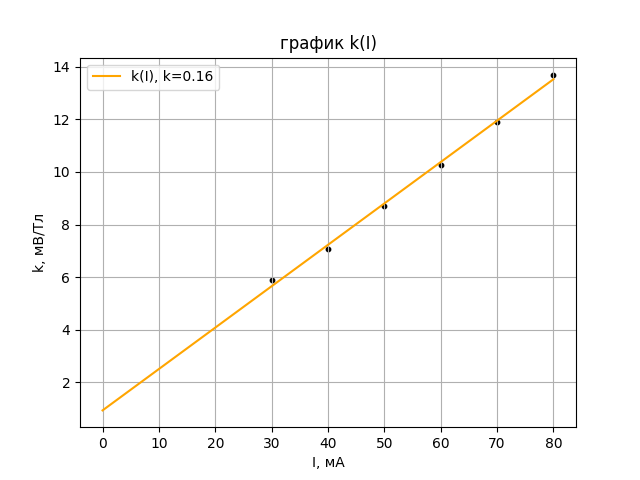
\includegraphics[width=1\linewidth]{graphs/figure3.png}
    \end{figure}
    
    \begin{figure}[H]
        \centering
        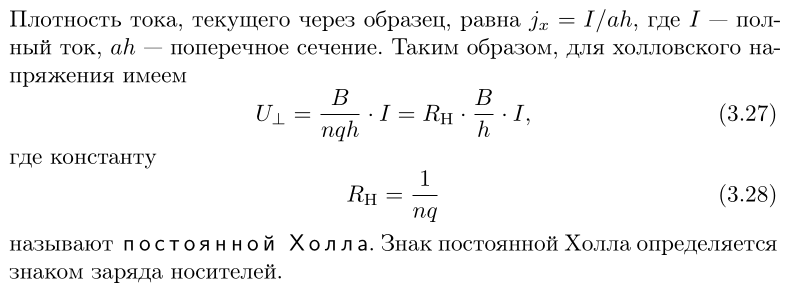
\includegraphics[width=1\linewidth]{images/theory.png}
    \end{figure}
    Отсюда получаем коэффициент Холла: $R_x = \frac{dk}{dI} \cdot h$, где h - толщины пластинки с током. \newline
    Отсюда с учетом МНК:
    $$R_x = 0.16 \cdot 0.0022 \approx 0.000032 = (0.32 \pm 0.02) \cdot 10^{-4} \frac{\text{м}^3}{\cdot \text{Кл}} $$

    Рассчитаем концентрацию носителей тока по формуле $n = \frac{1}{R_x e}$:
    $$n = \frac{1}{(0.32 \pm 0.02) \cdot 10^{-4} \cdot 1.6 \cdot 10^{-19}} \approx (1.85 \pm 0.15) \cdot 10^{21} \, \text{м}^{-3}$$

    Рассчитаем удельную проводимость исследуемого образца по формуле $\sigma = \frac{I L_{35}}{U_{35} a l}$ для I = 80 мА, $U_{35}$ = 65.21 мВ, $L_{35}$ = 15 мм, a = 2 мм, l = 8 мм:
    $$\sigma = \frac{0.08 \cdot 0.015}{0.06521 \cdot 0.002 \cdot 0.008} \approx (493 \pm 25) \, \frac{1}{\text{Ом} \cdot \text{м}}$$

    Подвижность электронов:
    $$b = \frac{\sigma}{en} = (157 \pm 18) \cdot 10^{-4}\frac{\text{м}^2}{\text{В}\cdot\text{с}}$$




\section{Обсуждение результатов}
    Мы изучили явление эффекта Холла в полупроводниках, измерили для нашего образца (Германий) такие величины как постоянная Холла, концентрацию электронов, удельную проводимость и подвижность электронов.
    \newpage
\onecolumn
\section{Приложение}

    \begin{table}[H] 
        \centering
        \begin{tabular}{|c|c|c|c|c|c|c|c|} \hline
        $I, \text{мA}$ & 0.3 & 0.6 & 0.9 & 1.2 & 1.5 & 1.8 & 2.1 \\ \hline
        \multicolumn{8}{|c|}{$I$ = 30 мА, $U_0$ = 0.11 мВ} \\ \hline
        $U, \text{мВ}$ & 1.33 & 2.24 & 3.17 & 3.93 & 4.43 & 4.76 & 5.04 \\ \hline
        $U_\bot, \text{мВ}$ & 1.22 & 2.13 & 3.06 & 3.82 & 4.32 & 4.65 & 4.93 \\ \hline
        \multicolumn{8}{|c|}{$I$ = 40 мА, $U_0$ = 0.18 мВ} \\ \hline
        $U, \text{мВ}$ & 1.25 & 2.56 & 3.72 & 4.76 & 5.43 & 5.86 & 6.25 \\ \hline
        $U_\bot, \text{мВ}$ & 1.07 & 2.38 & 3.54 & 4.58 & 5.25 & 5.68 & 6.07 \\ \hline
        \multicolumn{8}{|c|}{$I$ = 50 мА, $U_0$ = 0.21 мВ} \\ \hline
        $U, \text{мВ}$ & 1.56 & 3.17 & 4.61 & 5.85 & 6.73 & 7.27 & 7.5 \\ \hline
        $U_\bot, \text{мВ}$ & 1.35 & 2.96 & 4.4 & 5.64 & 6.52 & 7.06 & 7.29 \\ \hline
        \multicolumn{8}{|c|}{$I$ = 60 мА, $U_0$ = 0.32 мВ} \\ \hline
        $U, \text{мВ}$ & 1.9 & 3.84 & 5.54 & 6.94 & 7.95 & 8.61 & 9.02\\ \hline
        $U_\bot, \text{мВ}$ & 1.58 & 3.52 & 5.22 & 6.62 & 7.63 & 8.29 & 8.7 \\ \hline
        \multicolumn{8}{|c|}{$I$ = 70 мА, $U_0$ = 0.38 мВ} \\ \hline
        $U, \text{мВ}$ & 2.12 & 4.32 & 6.41 & 8.08 & 9.23 & 10.01 & 10.46\\ \hline
        $U_\bot, \text{мВ}$ & 1.74 & 3.94 & 6.03 & 7.7 & 8.85 & 9.63 & 10.08 \\ \hline
        \multicolumn{8}{|c|}{$I$ = 80 мА, $U_0$ = 0.39 мВ} \\ \hline
        $U, \text{мВ}$ & 2.45 & 5.09 & 7.31 & 9.19 & 10.59 & 11.46 & 11.96\\ \hline
        $U_\bot, \text{мВ}$ & 2.06 & 4.7 & 6.92 & 8.8 & 10.2 & 11.07 & 11.57 \\ \hline
        \end{tabular}
        \caption{Зависимость напряжения в образце от тока в обмотке электромагнита}
    \end{table}

\end{document}